\chapter{Accès à la ressource taille dépendant et compétition par interférence :
Analyse de séries temporelles longues de populations de collemboles \textit{Folsomia candida}}
\chaptermark{Analyse de séries temporelles structurées}
\label{chap:sp}

\vspace{3cm}
Voir Annexe \ref{Ann:SP}.
\vspace{1.5cm}

\lettrine[lines=3]{A}{ujourd'hui}, les conséquences de la compétition par
interférence sur les populations physiologiquement structurées, et plus
particulièrement les populations structurées en taille, restent assez peu
explorées. Nous présenterons dans ce chapitre les résultats d'une étude
expérimentale au cours de la quelle nous avons suivi 28 populations de
collemboles \textit{Folsomia candida} pendant $800$ à $1200$ jours. Cette étude
nous a permis d'en apprendre d'avantage sur le rôle que joue la structure des
populations à un instant donné sur la détermination de sa dynamique. Durant
cette étude, nous avons dénombré et mesuré la structure détaillée de $12$
populations du clone TO et $16$ populations du clone HA. Nous avons ensuite
réalisé une analyse qualitative et quantitative des séries temporelles obtenues
afin de relier les états (les structures) passés et présents de chaque
population avec sa dynamique future.
En particulier, cette étude nous a permis de mieux comprendre le rôle essentiel
que joue la présence d'individus de grande taille dans la régulation de la
dynamique des populations et de leur structure.

Les travaux présentés dans ce chapitre sont en cours d'écriture pour
publication, et peuvent être retrouvés dans l'Annexe \ref{Ann:SP}.

\section{Éléments de méthodologie}

\subsection{Conditions d'élevage et mesures des populations}

Nous avons élevé 28 populations de deux clones de
collemboles \textit{Folsomia candida} dans les conditions décrites dans le
Chapitre \ref{chap:method}: $12$ populations du clone
TO et $16$ populations du clone HA. Pour chaque population les mesures de nombre
d'individus et de structure en taille des populations ont été réalisées toutes
les unes à deux semaines en suivant la méthode automatisée décrite dans le
Chapitre \ref{chap:method}, Section \ref{sec:bpsensor} (voir aussi Annexe
\ref{Ann:bpsensor}).

\subsection{Analyse qualitative des séries temporelles}

Nous nous sommes d'abord intéressés aux dynamiques sur le long
terme de la structure des populations. Nous avons étudié de manière
qualitative ces dynamiques en traçant les séries temporelles structurées sur des
diagrammes structure-temps afin de faire ressortir le maximum d'information sur
la dynamique de la structure.
Nous avons alors séparé notre analyse en deux temps.

\subsubsection{Etat de la population}

Dans un premier temps, nous avons regardé la structure en taille des populations
de manière globale afin de repérer les structures caractéristiques que l'on
pouvait observer, sans considérer les dynamiques de court terme. Nous décrivons
alors plusieurs structures typiques différentes suivant le clone considéré et le
niveau de densité de la population.

\subsubsection{Dynamique de la structure de la population}

Dans un second temps, nous nous sommes attachés à décrire les dynamiques
temporaires que l'on peut observer sur les diagrammes structure-temps. Nous
avons essayé de déterminer des motifs dynamiques que l'on pouvait rattacher à
certains types de structures de populations, telles que celles décrites au
par-avant, ou à certains changements dans ces structures.

\subsection{Analyse quantitative des dynamiques des populations}

Suite à la description qualitative des dynamiques, nous avons réalisé une
analyse quantitative des structures observées et de leur dynamique. 

\subsubsection{Analyse en composante principale}

A chaque date de mesure, les données comprennent le nombre d'individus et pour
chaque individu sa longueur corporelle. Nous avons regroupé les données de
l'ensemble des populations à toutes les dates de mesures et nous avons
discrétisé la taille en classes de $0.1mm$ de $0$ à $3mm$. Nous obtenons ainsi
un tableau de données de $3341$ lignes (une ligne par classe de taille par date
par population) et $30$ colonnes. Chacune des colonnes peut alors être
considérée comme un vecteur de base dans l'espace à $30$ dimensions qui constitue l'espace
des structures de nos populations, et chaque ligne comme une observation dans
cet espace. Étant donnée la différence d'ordre de grandeur dans les nombres
d'individus entre juvéniles et adultes, nous avons utilisé le logarithme des
nombres d'individus dans chacune des classes de taille.

Malgré l'autocorrélation évidente de nos données, nous considérons chaque ligne
de notre tableau comme indépendante afin de mettre en évidence les motifs
récurrents de structure indépendamment de la population considérée. L'aspect
temporel des données sera réintroduit lors de l'étude des trajectoires dans
l'espace des composantes principales. Nous avons alors réalisé une analyse en
composantes principales (ACP) de nos données compilées.
Cela nous a permis d'extraire les quelques premières composantes et les vecteurs
et valeurs propres correspondantes. Ainsi, en ne conservant que peu de
composantes, on obtient une représentation condensée à quelques dimensions (deux
ou trois dans notre cas) des données de départ. Nous avons alors projeté chacune
des dynamiques de la structure des populations sur les deux premières
composantes de la décomposition. Un point dans l'espace à deux dimensions
représente alors une condensation de la structure d'une population à une date donnée.

\subsubsection{Regroupement non hiérarchique et projection sur les premières
composantes}

Parallèlement à l'ACP, nous avons effectué un regroupement non hiérarchique par
l'algorithme des ``k-means'' de nos données compilées. Ceci permet de regrouper
ensemble les structures de populations qui partagent des caractéristiques
communes, indépendamment de la date de mesure, du clone ou de la dynamique de la
population. Ainsi, nous avons pu déterminer quatre groupes cohérents de
structures de populations et identifier leurs caractéristiques précises. Une
fois projetés sur les deux premières composantes de l'ACP, les groupes obtenus
délimitent quatre régions distinctes du plan, confirmant ainsi la cohérence du
regroupement. 
 
\subsubsection{Dynamique des populations}

La visualisation des données sur le plan des deux premières composantes de l'ACP
et le regroupement en quatre types de structures permettent de représenter la
dynamique de la structure des populations par une trajectoire dans ce plan.
Cette trajectoire permet alors une analyse objective des dynamiques en
déterminant par exemple des temps de résidence dans chacune des structures type,
les nombres de transitions entre différentes structures types et la direction de
ces transitions. 

\section{Résultats}

Nous présenterons ici l'analyse détaillée de la dynamique de quatre populations,
deux du clone TO et deux du clone HA, ainsi que les résultats de l'analyse de l'ensemble des
populations. L'analyse graphique de chacune des populations est disponible à la
fin de l'article en Annexe \ref{Ann:SP} page \pageref{Ann:SP}. 

\subsection{Etude descriptive}

\subsubsection{Etats des populations}

La première partie de cette étude concerne une description qualitative des
périodes stables de la structure des populations (Figure \ref{fig:SP1}). On
appellera état des populations ces structures caractéristiques que l'on retrouve dans les
différentes populations. 

\begin{figure}[!ht]
\begin{center}
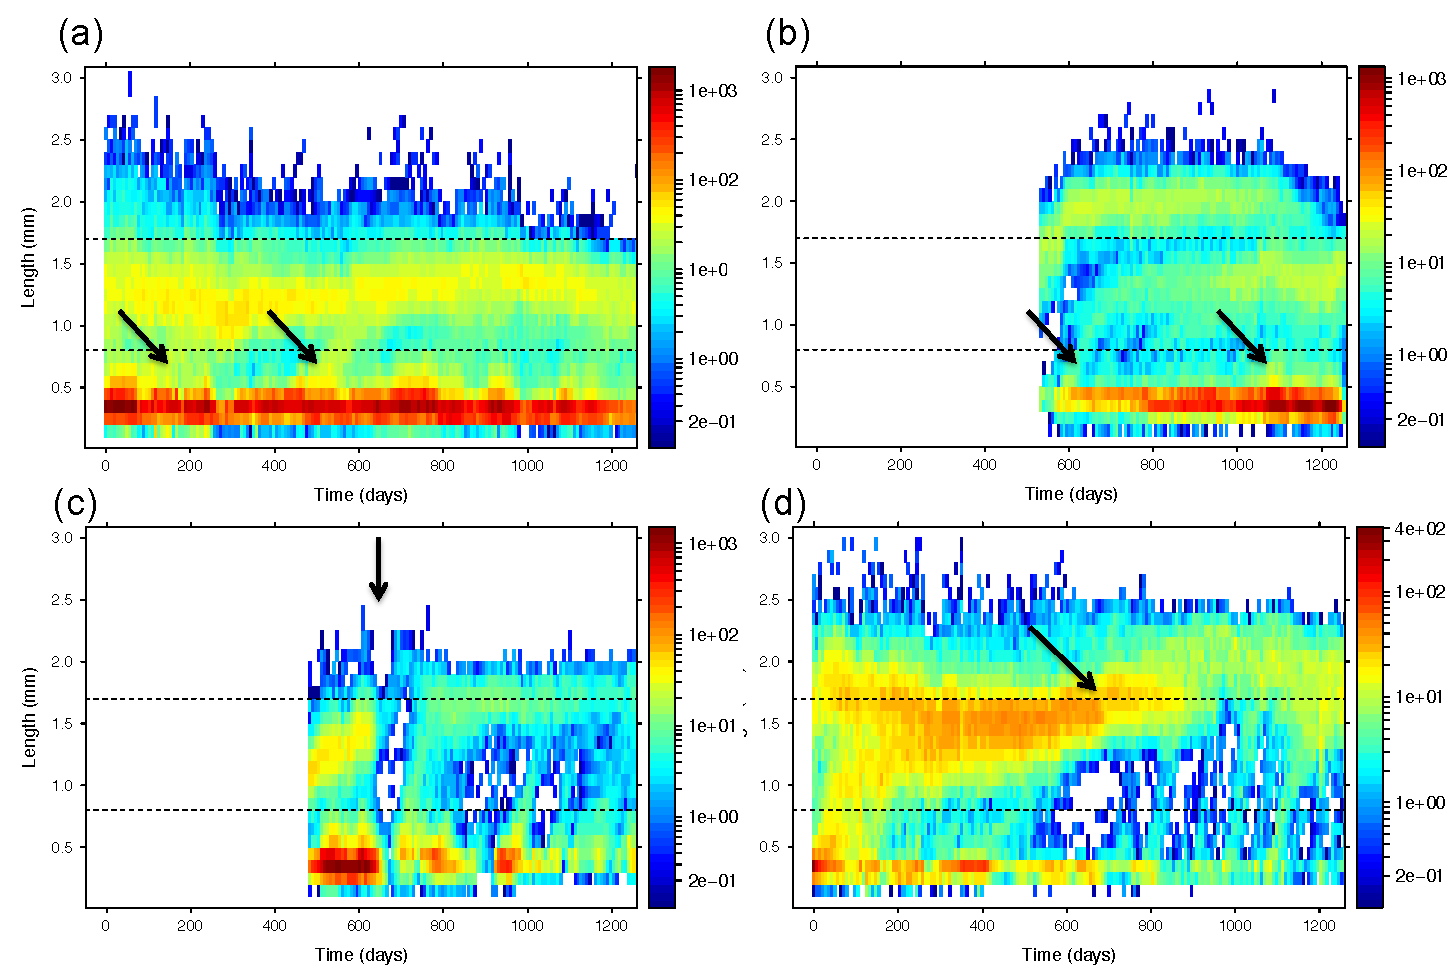
\includegraphics[width=0.95\textwidth]{1_CorpsDeThese/Resumes/Fig/SP01}
\caption[\lofimage{1_CorpsDeThese/Resumes/Fig/SP01}Dynamiques de la
structure de 4 populations]{Dynamique de la structure de quatre populations de
collemboles. (a) Clone TO, réplicat 3. (b) Clone HA, réplicat 15. (c) Clone TO,
réplicat 11. (d) Clone HA, réplicat 4. Les flèches noires en (a) et (b) montrent
des périodes de recrutement. Les flèches noires de (c) et (d) montrent des
événements conduisant à un nouveau recrutement, respectivement une catastrophe
(c) et la sénescence de la cohorte d'adultes (d).}
\label{fig:SP1}
\end{center}
\end{figure}

Les Figures \ref{fig:SP1}a et b montrent deux populations aux structures
relativement stables, mais dont la distribution en taille diffère. Dans le
premier cas, on constate que la distribution de la taille est fortement
bi-modale avec un groupe de juvéniles très dense ($>700$ individus de moins de
$0.5mm$) et un groupe d'adultes  moins dense ($<250$ individus de plus de
$0.8mm$), et avec très peu d'individus de taille intermédiaire. Dans le second
cas, on retrouve ces deux groupes pendant la totalité de la série temporelle, mais avec une
longue période pendant la quelle un troisième groupe de très grands adultes
subsiste ($>1.2mm$). Ces distributions multi-modales sont observées dans toutes
les populations étudiées. La plupart des populations ont une structure bi-modale,
plus ou moins stable dans le temps, tandis que certaines populations montrent
une structure tri-modale, exclusivement chez le clone HA. Le clone HA est donc
capable de produire des adultes de très grande taille à la survie très longue,
ce que TO est incapable de faire.

\subsubsection{Dynamique de la structure}

Dans un second temps, on s'intéresse aux événements dynamiques rapides
à l'échelle des séries temporelles. En effet, même si la structure peut être
relativement stable (Figure \ref{fig:SP1}a et b), on peut observer que des
processus dynamiques sont à l'\oe{}uvre.
 
\paragraph{Recrutement de cohortes}

Un premier processus remarquable est le recrutement de juvéniles dans les
classes d'adultes (flèches sur les Figures \ref{fig:SP1}a et b). Ces périodes de
recrutement  durent entre quelques dizaines et quelques centaines de jours.
Elles sont plus ou moins fréquentes, mais sont observées dans l'ensemble des
populations étudiées. On constate sur la Figure \ref{fig:SP1}b que ces recrutements
n'atteignent jamais la cohorte d'adultes les plus grands.
Ceci est vrai pour toutes les populations dans lesquelles un groupe d'adultes
de très grande taille subsiste. Lorsque ces individus géants sont présents dans
une population, il semble alors impossible pour les autres de grandir jusqu'à
ces tailles.

Ces périodes de recrutement permettent également d'estimer des taux de
croissance corporelle en fonction des conditions de la population (clone et
densité dans les différentes classes) en mesurant la pente de la cohorte qui
recrute. Ainsi, le taux de croissance de la cohorte marquée par la seconde
flèche de la Figure \ref{fig:SP1}a est d'environ $5\cdot 10^{-3}mm/j$, soit
$1mm$ tous les 200 jours. L'étude de ces taux de croissance en fonction de la
densité et des conditions de température fera l'objet du Chapitre \ref{chap:fip}
et de l'Annexe \ref{Ann:fip}.

Ces périodes de recrutement surviennent parfois à la suite d'événements
catastrophiques. On constate sur la Figure \ref{fig:SP1}c (flèche) que c'est
après la disparition brutale et quasi-totale des adultes que survient un des
plus gros recrutements d'individus de la série temporelle. Ceci se retrouve
également sur d'autres populations (voir Table \ref{tab:SP}). Ainsi, la
disparition brutale des adultes de la population déclenche le recrutement de
nouveaux individus chez les adultes. 

Enfin, le recrutement de nouvelles cohortes de juvéniles peut également
intervenir après le déclin naturel du groupe d'adultes, soit chez le groupe de
géants (Figure \ref{fig:SP1}b, seconde flèche), soit le seul groupe présent
(Figure \ref{fig:SP1}d, flèche). On constate par exemple dans le second cas que
pendant une très longue période la population est composée de quelques jeunes et
d'une très large cohorte d'adulte, avec très peu de recrutement de nouveaux
adultes. Ce groupe d'adulte décline au cours du temps, et lorsqu'il a
suffisamment diminué en densité (aux environs de $800$ jours, flèche), des
recrutements de jeunes commencent à survenir. Ceci confirme le rôle des
adultes de plus grande taille dans le contrôle de la dynamique de la structure
et le renouvellement des populations. 

\paragraph{Plasticité de la taille adulte}

L'étude de ces séries temporelles révèle également des ajustements de la taille
des adultes au cours des différents événements décrits précédemment. Tout
d'abord, suivant les conditions démographiques, les cohortes d'adultes se
stabilisent à différentes tailles. Les populations montrées en exemple sur la
Figure \ref{fig:SP1} montrent chacune une taille d'équilibre différente. En
particulier, la taille adulte a tendance à être plus grande quand la densité
de la population est plus faible. Ce point fera également l'objet d'une étude
approfondie dans le Chapitre \ref{chap:fip} (voir aussi Annexe \ref{Ann:fip}).

De plus, les individus sont capables d'ajuster rapidement leur taille corporelle
en fonction des changements de conditions environnementales et démographiques.
Après la chute catastrophique de la cohorte d'adultes montrée Figure
\ref{fig:SP1}c, les adultes survivants reprennent une croissance très rapide sur
une courte durée (augmentation de près de $40\%$ de leur taille corporelle en
quelques semaines).
De même dans le cas de la sénescence des adultes (Figure \ref{fig:SP1}d), les
adultes restant grandissent de $1.7mm$ à près de $2.2mm$.

De façon plus étonnante, les adultes sont également capables de diminuer leur
taille corporelle. Par exemple au cours des $200$ premiers jours sur la Figure
\ref{fig:SP1}d où la taille des adultes diminue pendant qu'une grande cohorte de
juvéniles atteint la maturité. Ces rétrécissements des adultes ont été observés
dans d'autres populations (HA réplicats 1 à 3, TO réplicats 5 et 9 par exemple).
La plasticité de la taille adulte des collemboles est décrite et étudiée par
\textcites{mallard2013b} dans ses travaux de thèse.

La Table \ref{tab:SP} résume les dates où les différents événements décrits ont
été observés dans les populations étudiées. 

{\tiny
\begin{longtable}{
	p{\dimexpr.12\linewidth-2\tabcolsep-1.3333\arrayrulewidth}% column 1
 	p{\dimexpr.128\linewidth-2\tabcolsep-1.3333\arrayrulewidth}
 	p{\dimexpr.128\linewidth-2\tabcolsep-1.3333\arrayrulewidth}% column 1
 	p{\dimexpr.128\linewidth-2\tabcolsep-1.3333\arrayrulewidth}
 	p{\dimexpr.12\linewidth-2\tabcolsep-1.3333\arrayrulewidth}% column 1
 	p{\dimexpr.12\linewidth-2\tabcolsep-1.3333\arrayrulewidth}
 	p{\dimexpr.126\linewidth-2\tabcolsep-1.3333\arrayrulewidth}% column 1
 	p{\dimexpr.126\linewidth-2\tabcolsep-1.3333\arrayrulewidth}}

\caption{Dates d'observations des états et dynamiques
 	décrites. Les nombres correspondent aux dates en jours ou aux
 	intervalles pendant lesquels les événements ont été
 	observés.\label{tab:SP}}\\
 	 	
 	\hline
 	\endhead
 	
\hline
\endfoot


 	
Populations & Structure Trimodale & Longue période sans recrutement &
Recrutement fréquent & Événement catastrophique & Sénescence de la cohorte adulte &
Croissance adulte d'ajustement & Rétrécissement adulte d'ajustement \\
\hline\\
HA r1 & - 			& - 		& - 		& - 	& 500  & 500-650  & 650-750  \\
HA r2 & - 			& - 		& - 		& - 	& 800  & 650-900  & - 		 \\
HA r3 & - 			& - 		& - 		& - 	& 800  & 900-1000 & 1000-1250\\
HA r4 & - 			& - 		& - 		& - 	& 800  & 600-1000 & -        \\
HA r5 & 600-1000 	& - 		& - 		& - 	& 1000 & - 		  & - \\
HA r6 & - 			& 800-1250 	& - 		& - 	& -    & - 		  & - \\
HA r7 & 700-1100 	& - 		& - 		& - 	& 1000 & - 		  & - \\
HA r8 & 600-1000 	& - 		& - 		& - 	& 950  & - 		  & - \\
HA r9 & 700-1200 	& 700-1100 	& - 		& - 	& -    & - 		  & - \\
HA 10 & 600-900 	& - 		& - 		& - 	& 900  & - 		  & - \\
HA 11 & 600-1100 	& 700-1250 	& - 		& - 	& 1100 & - 		  & - \\
HA 12 & 600-900 	& - 		& 600-1250 	& - 	& 1000 & - 		  & - \\
HA 13 & 600-1100 	& - 		& 600-1250 	& - 	& 1100 & - 		  & - \\
HA 14 & 600-1100 	& 600-1000 	& - 		& - 	& 1100 & - 		  & - \\
HA 15 & 600-1100 	& - 		& 600-1250 	& - 	& 1100 & - 		  & - \\
HA 16 & 600-1200 	& - 		& - 		& - 	& 1200 & - 		  & - \\
TO r1 & - 			& 400-600 	& 0-400 	& - 	& 400  & 400-600  & -\\
	  &				& 700-1000	& 1000-1250 & 		&	   &		  &\\
TO r2 & - 			& 500-750 	& 0-450 	& - 	& 400  & 500-700  & - \\
	  & 			& 			& 1000-1250 &		&	   &		  &\\
TO r3 & - 			& 600-1250 	& - 		& - 	& -    & - 		  & 0-200\\
TO r4 & - 			& - 		& 0-1250	& - 	& 400  & - 		  & 700-1000\\
TO r5 & - 			& - 		& - 		& 900 	& -    & 900-1000 & 500-700\\
TO r6 & - 			& 600-950 	& - 		& 950 	& -    & 950-1000 & -\\
TO r7 & - 			& - 		& 500-1250 	& - 	& -    & - 		  & -\\
TO r8 & - 			& 600-800 	& 800-1250 	& - 	& 1000 & 1000-1100& -\\
TO r9 & - 			& 600-1000 	& - 		& - 	& 950  & 900-1000 & 500-600\\
TO 11 & - 			& - 		& 700-1250 	& 650 	& -    & 650-750  & -\\
TO 12 & - 			& - 		& - 		& 750 	& -    & 750-850  & -\\
TO 13 & - 			& 500-800 	& 800-1250 	& 800 	& -    & - 		  & -\\

\end{longtable}
}

\subsection{Analyse quantitative des dynamiques}

\subsubsection{Composantes principales}

\begin{figure}[!ht]
\begin{center}
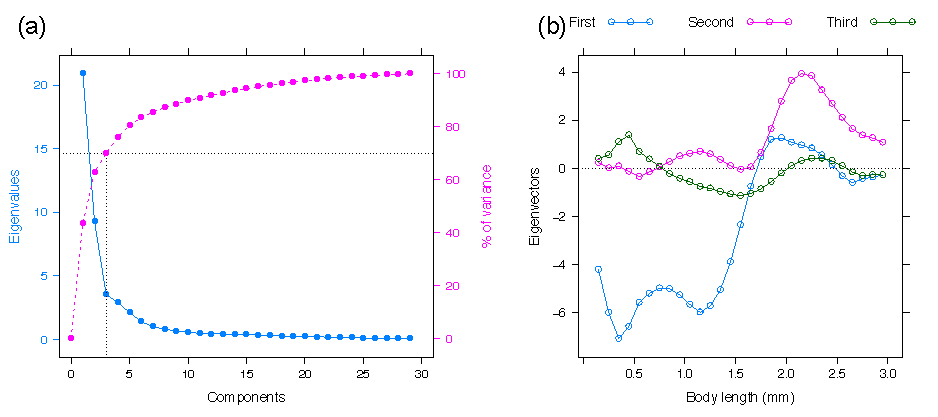
\includegraphics[width=0.95\textwidth]{1_CorpsDeThese/Resumes/Fig/SP02}
\caption[\lofimage{1_CorpsDeThese/Resumes/Fig/SP02}Composantes
principales]{(a) Scree plot de l'ACP. La ligne bleue pleine donne les valeurs
propres, la ligne pointillée donne le pourcentage cumulé de variance expliquée.
(b) Coordonnées des trois premiers vecteurs propres.}
\label{fig:SP2}
\end{center}
\end{figure}

La Figure \ref{fig:SP2}a représente les valeurs propres de l'ACP et le
pourcentage cumulé de variance expliquée. On observe une cassure nette après la
troisième composante, les trois premières composantes expliquant $70\%$ de la
variance totale. Cela montre que les trois premières composantes permettent
d'expliquer l'essentiel des variations entre les structures dans nos différentes
populations. La Figure \ref{fig:SP2}b montre que les variations expliquées
par ces trois composantes se répartissent sur l'ensemble de l'espace de départ,
sans classe de taille non expliquée.
En particulier, la première composante expliquant $43\%$ de la variance
correspond essentiellement aux variations dans les individus de moins de
$1.5mm$. La seconde composante quant à elle, qui représente $20\%$ de la
variance explique une partie des variations des petits adultes ($0.8$ à
$1.3mm$), et principalement au niveau des individus de plus de $1.6mm$. La troisième
composante permet de distinguer les individus de taille
intermédiaire ($0.8$ à $1.9mm$) et les petits individus ($<0.8mm$). Ces trois
composantes permettent de définir plusieurs groupes de classes de taille sans a
priori: (i) les juvéniles ($<0.6mm$), négatifs sur le premier axe et positif sur
le troisième; (ii) les petits adultes (entre $0.6$ et $1.2mm$) positifs sur le
second axe, négatifs sur les autres; (iii) les adultes intermédiaires ($1.2$ à
$1.9mm$) négatifs sur le troisième axe; et (iv) les grands adultes ($>1.9mm$),
positifs sur le second axe. Ces groupes recoupent bien la description
qualitative des diagrammes mais sans a priori sur les limites entre groupes.

Les deux premières composantes représentant $63\%$ de la variance, nous ne
conserveront pas la troisième composante dans la suite de l'étude. Cela nous
permettra une représentation graphique simplifiée des structures des populations
dans le plan des deux premières composantes. 

\subsubsection{Groupement non hiérarchique}

En utilisant l'algorithme des ``k-means'', nous avons regroupé les structures
qui partageaient des caractéristiques communes en quatre groupes. En traçant ces
structures ensemble, nous avons pu déterminer quatre grandes structures typiques
de populations expérimentales (Figure \ref{fig:SP3a}): (i) une
structure avec beaucoup de juvéniles et des adultes de petite taille (type $1$);
(ii) une structure avec des adultes de taille intermédiaire (type $2$); (iii)
une structure avec moins de juvéniles et des adultes de grande taille (type
$3$); et (iv) une structure trimodale avec des juvéniles, des petits et des
grands adultes (type $4$).

\begin{figure}[!ht]
\begin{center}
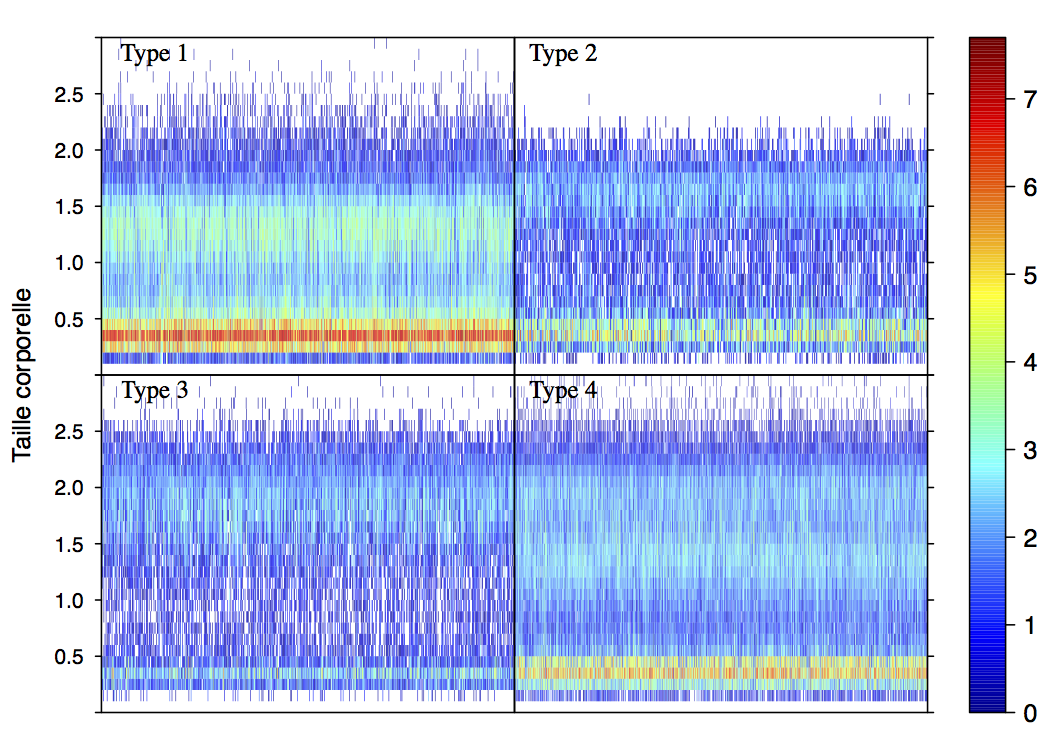
\includegraphics[width=0.95\textwidth]{1_CorpsDeThese/Resumes/Fig/SP02c}
\caption[\lofimage{1_CorpsDeThese/Resumes/Fig/SP02b}Quatres grands
types de structures]{Structures caractéristiques des quatre grands types de
structure identifiés.}
\label{fig:SP3a}
\end{center}
\end{figure}

En projetant la structure de chacune des populations à chaque date de mesure
sur les deux premières composantes de l'ACP, et en séparant les points en
fonction du type de structure auquel ils appartiennent, on constate que la
séparation en quatre groupes reste remarquablement cohérente dans l'espace
réduit à deux dimensions (Figure \ref{fig:SP3}), et délimitent quatre régions
distinctes du plan.

\begin{figure}[!ht]
\begin{center}
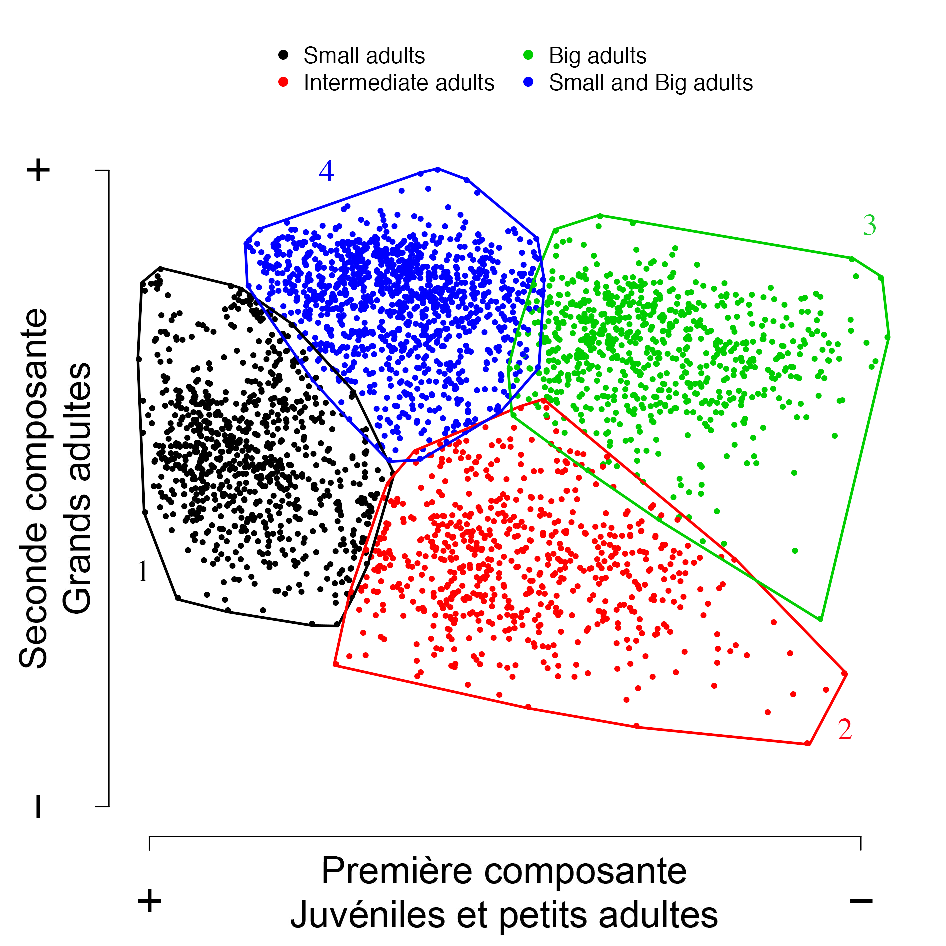
\includegraphics[width=0.75\textwidth]{1_CorpsDeThese/Resumes/Fig/SP03b}
\caption[\lofimage{1_CorpsDeThese/Resumes/Fig/SP03b}Projection des données
sur les deux premières composantes]{Projection des structures sur les deux
premières composantes de l'ACP et groupement en 4 types de structure. Les
domaines délimités seront reportés sur les trajectoires temporelles dans le
plan des deux premières composantes.}
\label{fig:SP3}
\end{center}
\end{figure}

Cette représentation permet une classification objective de la structure d'une
population à un temps donné dans un des quatre types de structure. Cela permet
aussi d'observer la trajectoire temporelle dans le plan des deux premières
composantes de l'ACP et donc sa dynamique entre les différentes structures caractéristiques. 

\subsubsection{Trajectoires dans le plan des composantes}

\begin{figure}[!ht]
\begin{center}
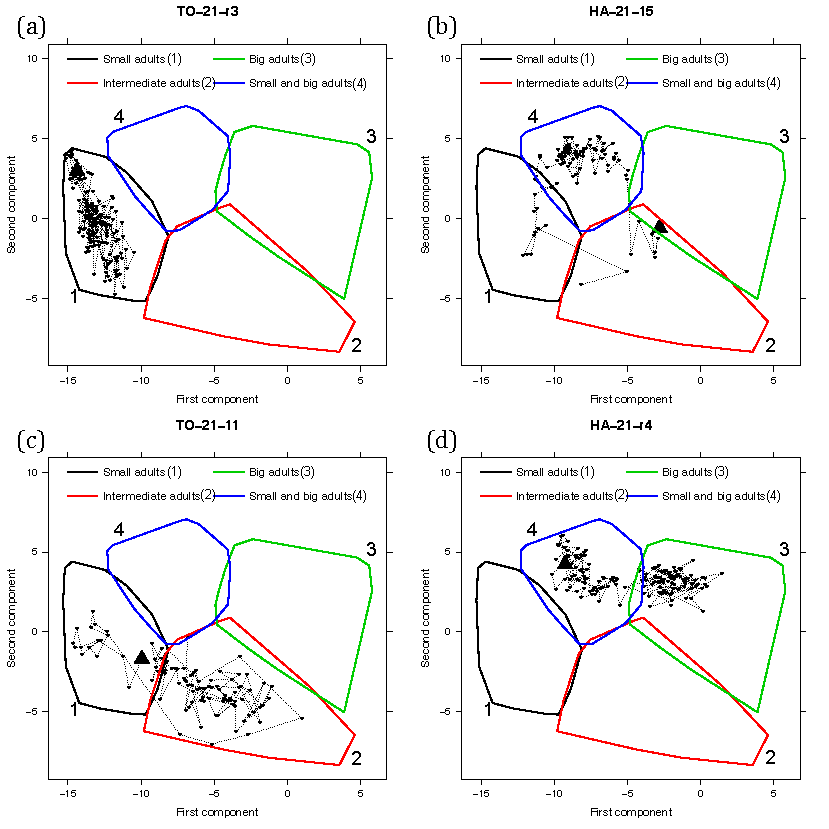
\includegraphics[width=0.95\textwidth]{1_CorpsDeThese/Resumes/Fig/SP04}
\caption[\lofimage{1_CorpsDeThese/Resumes/Fig/SP04}Trajectoires des
popualtions exemple dans le plan des composantes]{Trajectoires des
populations exemples dans le plan des composantes. Les lignes colorées et
numérotées représentes les quatre grands types de structure issus de la
classification non hiérarchique. Chaque points est une mesure de structure à
une date donnée. Le triangle représente le début de la trajectoire. Les lignes
pointillées relient chronologiquement les points.}
\label{fig:SP4}
\end{center}
\end{figure}

La Figure \ref{fig:SP4} montre les mêmes populations que sur les diagrammes
structure-temps de la Figure \ref{fig:SP1}, en projetant les structures dans le
plan des deux premières composantes. Cette représentation permet de confirmer
numériquement que la population TO 3 (Figures \ref{fig:SP1}a et \ref{fig:SP4}a)
reste tout le temps dans une structure de type 1 alors que la population TO 11
(Figures \ref{fig:SP1}c et \ref{fig:SP4}c) débute dans une structure de type 1
mais converge finalement vers une structure de type 2 avec moins de juvéniles et
des adultes plus grands. De même pour les populations HA  (Figures
\ref{fig:SP1}bd et \ref{fig:SP4}bd) qui restent toutes les deux dans une
configuration de type 4 trimodale avant de basculer, l'une vers une structure de
type 2 avec des adultes petits à intermédiaires (panel b), l'autre vers une
structure de type 3 avec des grands adultes (panel d).

\subsubsection{Stabilité des structures et transitions}

L'ACP et la projection des dynamiques sur les deux premières composantes
permettent de mesurer des temps de résidence dans chacun des quatre types de
structure, et des transitions entre les grands types. Par exemple, alors que la
population TO 3 (Figures \ref{fig:SP1}a et \ref{fig:SP4}a) est très stable et
passe 1200 jours dans le même type de structure, les autres populations ont
tendance avoir des transitions entre plusieurs types de structures. En
particulier, la population HA 15 (panel b) a une phase transitoire d'une
cinquantaine de jours en type 2 avant de se stabiliser en type 4 pendant 550
jours, puis de revenir en type 2. En conduisant la même analyse sur chacune des
28 populations, nous pouvons alors étudier la distribution du temps passé dans
chacune des régions par chacun des clones. 

\begin{figure}[!ht]
\begin{center}
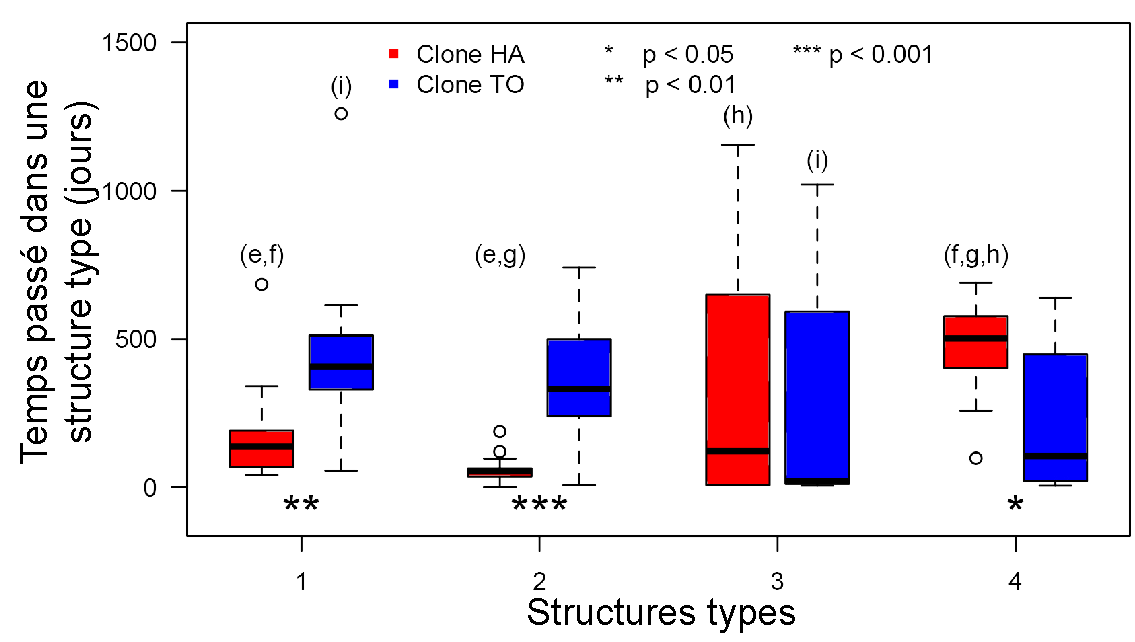
\includegraphics[width=0.95\textwidth]{1_CorpsDeThese/Resumes/Fig/SP05}
\caption[\lofimage{1_CorpsDeThese/Resumes/Fig/SP05}Temps de
résidence dans les structures types]{Temps passé dans chacun des types de
structure caractéristique suivant les clones. Les lettres montrent les
différences significatives dans les distributions (Tests de Kolmogorov-Smirnov
à deux échantillons: (e) D=0.54, p=0.02, (f) D=0.78, p=0.0003, (g) D=0.93,
p=3x10-6, (h) D=0.53, p=0.03, (i) D=0.67, p=0.04). Les étoiles montrent les
différences significatives entre clones dans un même type de structure.}
\label{fig:SP5}
\end{center}
\end{figure}

On constate alors que les différents types de structures ne sont pas toutes
aussi stables (Figure \ref{fig:SP5}). Ainsi, bien que la variabilité soit très grande,
les temps de résidence les plus longs observés sont dans le type 3, avec des
adultes de grande taille.
Ces adultes de grande taille ont une très grande longévité et subissent peu de
compétition de la part des autres individus, ce qui a un effet stabilisant sur
la structure de la population. Cet effet est également visible pour les
structures trimodales (type 4) où les temps de résidences sont également très
long. A l'opposé, les structures de types 2 sont les moins stables, en effet,
les adultes intermédiaires vont être soit exclus compétitivement par les plus
petits, ce qui fait revenir la population en type 1, soit plus fréquemment
continuer à grandir, ce qui fait basculer la population en type 3.

On constate également qu'il existe des différences marquées entre clones. Ainsi,
TO passe plus de temps dans les structures de type 1 et 2 où les adultes sont
plus petits et la densité de juvéniles est importante, alors que HA est plus
souvent dans une structure de type 3 ou 4 avec des adultes de très grande taille
et moins de juvéniles. Cela reflète des stratégies d'histoire de vie différentes
des clones TO et HA, le premier ayant tendance à privilégier la reproduction sur
la croissance, alors que le second privilégie la croissance sur la reproduction.

\section{Discussion}

\subsection{Conséquences des différences génétiques sur la dynamique des
populations}

Les différences de stratégies d'histoires de vie peuvent avoir un effet très
fort sur la dynamique des populations via notamment deux facteurs. Le premier
est sur la réponse à la compétition, en effet les juvéniles sont plus
compétitifs dans le cas de l'exploitation alors que les grands adultes sont supérieurs dans
le cas de l'interférence. Le second concerne la réponse à des changements de
températures puisqu'on a vu que ces derniers pouvaient affecter la taille
individuelle et les structures des populations. Les deux clones étudiés sont
connus pour leurs stratégies différentes \autocites{tully2006a,tully2008a}, TO
étant très flexible dans son investissement reproducteur au détriment de sa
taille corporelle, alors que HA l'est moins mais atteint des plus
grandes tailles.

Ces différences affectent la dynamique de la structure des populations puisque
la faible flexibilité de HA et sa capacité à produire des adultes de grande
taille lui permettent d'atteindre des structures de type 3 voir 4 très
stables alors que TO reste dans des structures de type 1 ou 2. Une
fois établis, les adultes de grande taille dominent la population et empêchent
les autres individus de grandir en monopolisant la ressource, ce qui amène
notamment à la stabilisation d'un groupe de petits adultes et des structures de
type 4 trimodales. Cela montre l'importance de connaître les stratégies
d'histoire de vie des espèces étudiées afin de comprendre correctement la
dynamique de leur structure et \textit{in fine} de prédire la dynamique de la
population dans son ensemble.

\subsubsection{Le rôle des conditions initiales}

Bien que la structure de type 4 semble très stable, il est intéressant de noter
qu'elle n'est visible qu'au début de certaines séries temporelles. En effet, ce
type de structure est très stable localement, mais n'est atteignable que dans
des conditions très particulières. Il est nécessaire: (i) que les individus
puissent grandir vite jusqu'à des très grandes tailles, ce qui est le cas
de HA mais pas de TO; et (ii) que le niveau de compétition soit à son minimum,
ce qui se traduit par une absence d'adulte dans la population, et une faible
densité de jeunes. Dans ces conditions, les jeunes présents vont alors grandir
jusqu'aux plus grandes tailles et commencer à se reproduire tout en monopolisant
la ressource, ce qui n'autorise les autres juvéniles à grandir que jusqu'à des
tailles intermédiaires. C'est par la sénescence de la cohorte d'adultes les plus
grands que la dynamique de la population peut quitter cet attracteur et
converger vers une structure de type 1, 2 ou 3.

Les autres types de structures dépendent aussi des conditions initiales. Une
forte densité de juvéniles comme condition initiale d'une population conduira à
une structure de type 1 alors qu'une distribution relativement homogène en
densité moyenne conduira à une structure de type 2 chez TO et de type 3 chez HA.
L'importance des conditions initiales montre la coexistence des quatre
attracteurs quasi-stables de la structure des populations. De plus, les
transitions entre ces attracteurs sont généralement dues soit à un événement
catastrophique, soit à la sénescence des adultes de grande taille. 

Enfin, cette sensibilité aux conditions initiales montre l'importance de
considérer la structure dans l'étude de la dynamique des populations. En effet,
bien que le nombre global d'individus  puisse être le même, une structure
différente pourra mener à des dynamiques très différentes. 
Cela va dans le sens des résultats de \textcites{benton2005a} sur la dynamique de populations
d'acariens structurées en âge montrant que des séquences données de changements
environnementaux peuvent amener à des dynamiques très différentes en fonction de
détails des conditions initiales de la structure en âge et de la densité des
populations.

\subsubsection{La compétition par interférence}

Nous avons montré à plusieurs reprises le rôle déterminant que jouent les
adultes de grande taille dans la dynamique de nos populations. Si l'accès à la ressource
n'était régulé que par la compétition par exploitation, tous les individus
parviendraient à accéder à la ressource, et la théorie du budget énergétique
dynamique nous prédit que les grands individus seraient exclus par les plus
petits, plus efficaces dans leur gestion de l'énergie
\autocites{kooijman1984a,de-roos1997a}. Dans ces conditions, les structures tendraient
vers une majorité de juvéniles et des adultes qui ne grandissent plus une fois la maturité atteinte. 

Or, nos dynamiques montrent clairement que les individus de grande taille
exercent une domination sur les populations: (i) certaines conditions permettent
l'émergence et le maintient à long terme de cohortes d'adultes géants; (ii) lors
de la disparition catastrophique d'une cohorte d'adultes, les juvéniles présents
commencent immédiatement à grandir; (iii) la sénescence d'une cohorte d'adultes
et sa disparition progressive se traduit aussi par une reprise de la croissance
des juvéniles; et (iv) des cohortes très denses d'adultes s'accompagnent
généralement de longues périodes sans recrutement. Ainsi, il semble que nos
populations soient régulées par la domination des adultes. Un mécanisme probable
permettant cette domination adulte serait la position privilégiée qu'ils
occupent dans l'accès à la ressource disponible, privant les plus petits
individus, les empêchant de grandir. Ceci est un mécanisme caractéristique de la
compétition par interférence. Lorsque le nombre d'adultes de grande taille
diminue, la pression de compétition est relâchée et les plus petits individus
parviennent de nouveau à accéder à la ressource et à se développer.


\section{En conclusion}

Cette étude montre que l'analyse de la dynamique temporelle de la
structure des populations permet d'accéder plus précisément aux mécanismes en
jeu dans leur régulation, tels que le rôle des stratégies individuelles
d'histoire de vie, ou le type d'interaction compétitive à l'oeuvre. Nous pensons
que cette étude est un exemple concret du fait qu'une population puisse être
contrôlée par ses adultes les plus grands, donnant lieu à des dynamiques
complexes qui dépendent directement des stratégies d'histoire de vie des
individus et des conditions environnementales, y compris la densité de
la population.
Modéliser le rôle de la compétition par interférence dans la dynamique des populations structurées, dans le cadre des modèles PSP, nous
permettra de confirmer son rôle essentiel dans la survie des
individus de grande taille, et dans l'émergence de dynamiques temporelles
impliquant des distributions de taille multi-modales (Chapitre
\ref{chap:amnat} et Annexe \ref{An:AmNat}).

De plus, il serait nécessaire de vérifier précisément le rôle joué par les
adultes, notamment pour confirmer leur domination dans l'accès aux ressources,
ce qui viendrait confirmer l'hypothèse de l'interférence comme mécanisme de
régulation des populations. Ceci fera l'objet d'une étude expérimentale
présentée dans le Chapitre \ref{chap:sm}.


